\documentclass[12pt]{article}
\usepackage[margin=1in]{geometry}
\usepackage{listings}
\usepackage{graphicx}
\usepackage{float}
\usepackage{color} %red, green, blue, yellow, cyan, magenta, black, white
\definecolor{mygreen}{RGB}{28,172,0} % color values Red, Green, Blue
\definecolor{mylilas}{RGB}{170,55,241}

\setlength{\parskip}{1em}

\lstset{language=Matlab,%
    %basicstyle=\color{red},
    breaklines=true,%
    morekeywords={matlab2tikz},
    keywordstyle=\color{blue},%
    morekeywords=[2]{1}, keywordstyle=[2]{\color{black}},
    identifierstyle=\color{black},%
    stringstyle=\color{mylilas},
    commentstyle=\color{mygreen},%
    showstringspaces=false,%without this there will be a symbol in the places where there is a space
    numbers=left,%
    numberstyle={\tiny \color{black}},% size of the numbers
    numbersep=9pt, % this defines how far the numbers are from the text
    emph=[1]{for,end,break},emphstyle=[1]\color{red}, %some words to emphasise
    %emph=[2]{word1,word2}, emphstyle=[2]{style},    
}

\usepackage{mathtools}
\usepackage{url}

\title{Assignment 4, COMP4702}
\author{Roy Portas, 43560846}
\date{\today}

\begin{document} 
\begin{titlepage}
    \maketitle
\end{titlepage}

\section*{Prac 10}

\subsection*{Question 3}

\begin{figure}[H]
    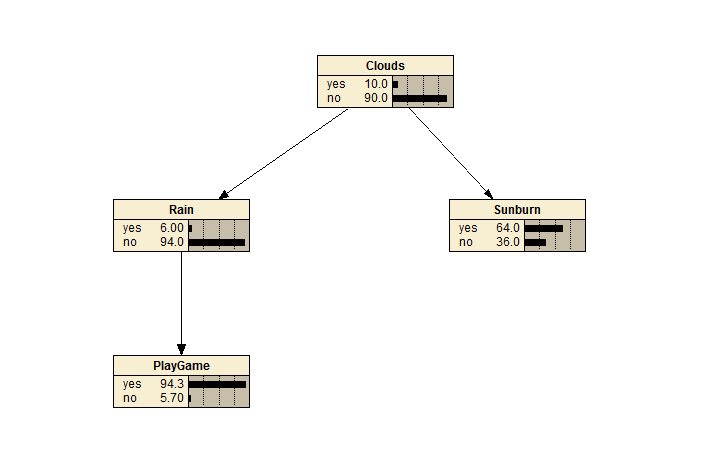
\includegraphics[width=\linewidth]{../../pracs/prac10/q3_network}
    \centering
    \caption{Network}
\end{figure}

The probabilities in the network match the course notes, thus are valid.

\begin{figure}[H]
    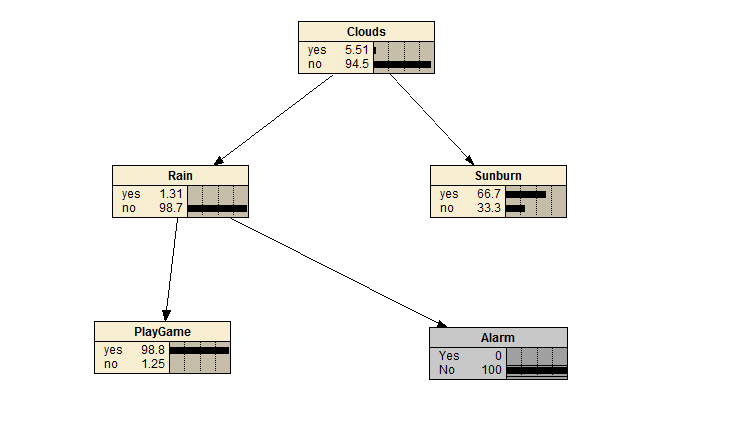
\includegraphics[width=\linewidth]{../../pracs/prac10/q3_no_rain}
    \centering
    \caption{No Alarm}
\end{figure}

If there is no rain alarm then the chance of clouds decrease by around a half, to 5.51\%.
Since the alarm is not going off, there is a 99.8\% chance the game will be played.
Additionally the chance of sunburn increases by around 3\%.

\subsection*{Question 4}

For this question Bayes rule is required.

\begin{align*}
    P(C|W) = \frac{P(W|C) P(C)}{P(W)}
\end{align*}

Thus three parts are required, $P(W|C)$, $P(C)$ and $P(W)$.

\begin{align*}
    P(C) &= 0.5\\
    P(\sim C) &= 0.5
\end{align*}

\begin{align*}
    P(W|C) &= P(W|RS) \times P(R|C) \times P(S|C)\\
    &\qquad+ P(W|\sim R S) \times P(\sim R|C) \times P(S|C)\\
    &\qquad+ P(W|R\sim S) \times P(R|C) \times P(\sim S | C)\\
    &\qquad  + P(W| \sim R \sim S) \times P(\sim R | C) \times P(\sim S | C)\\
    &= 0.95 \times 0.8 \times 0.1\\
    &\qquad + 0.9 \times 0.2 \times 0.1\\
    &\qquad + 0.9 \times 0.8 \times 0.9\\
    &\qquad + 0.1 \times 0.2 \times 0.9\\
    &= 0.076 + 0.018 + 0.648 + 0.018\\
    &= 0.76
\end{align*}

\begin{align*}
    P(W|\sim{C}) &= P(W|RS) \times P(R|\sim{C}) \times P(S|\sim{C})\\
    &\qquad+ P(W|\sim{R}S) \times P(\sim{R}|\sim{C}) \times P(S|\sim{C})\\
    &\qquad+ P(W|R\sim{S}) \times P(R|\sim{C}) \times P(\sim{S}|\sim{C})\\
    &\qquad+ P(W|\sim{R}\sim{S}) \times P(\sim{R}|\sim{C}) \times P(\sim{S}|\sim{C})\\
    &= 0.95 \times 0.1 \times 0.5\\
    &\qquad+ 0.9 \times 0.9 \times 0.5\\
    &\qquad+ 0.9 \times 0.1 \times 0.5\\
    &\qquad+ 0.1 \times 0.9 \times 0.5\\
    &= 0.0475 + 0.405 + 0.045 + 0.045\\
    &= 0.5425
\end{align*}

\begin{align*}
    P(W) &= P(W|C) \times P(C) + P(W|\sim C) \times P(\sim C)\\
    &= 0.76 \times 0.5 + 0.5425 \times 0.5\\
    &= 0.65125
\end{align*}

Combining this all together yields the following

\begin{align*}
    P(C|W) &= \frac{P(W|C) P(C)}{P(W)}\\
    &= \frac{0.76 \times 0.5}{0.65125}\\
    &= 0.583493
\end{align*}

Thus the probablity that it is cloudy given the grass is wet is $0.583$ or $58.3\%$.

\begin{figure}[H]
    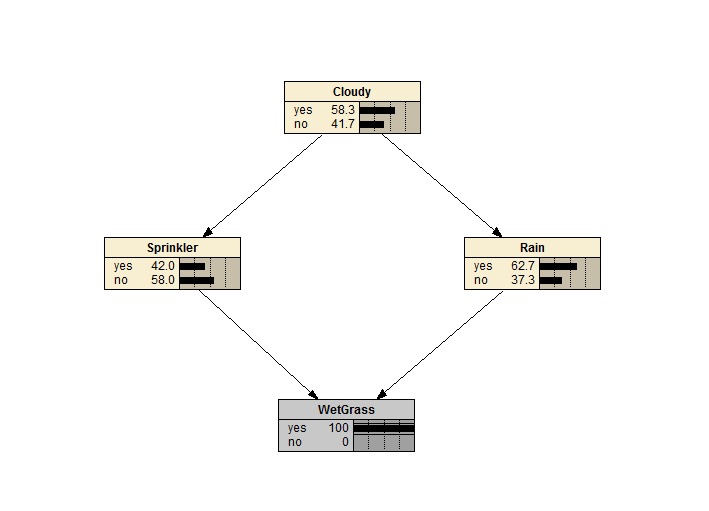
\includegraphics[width=\linewidth]{../../pracs/prac10/q4}
    \centering
    \caption{Network}
\end{figure}

This matches the value given by the equations, which is $58.3\%$.

\section*{Prac 11}

\subsection*{Question 1}

\lstinputlisting[language=Matlab]{../../pracs/prac11/q1.m}

\begin{figure}[H]
    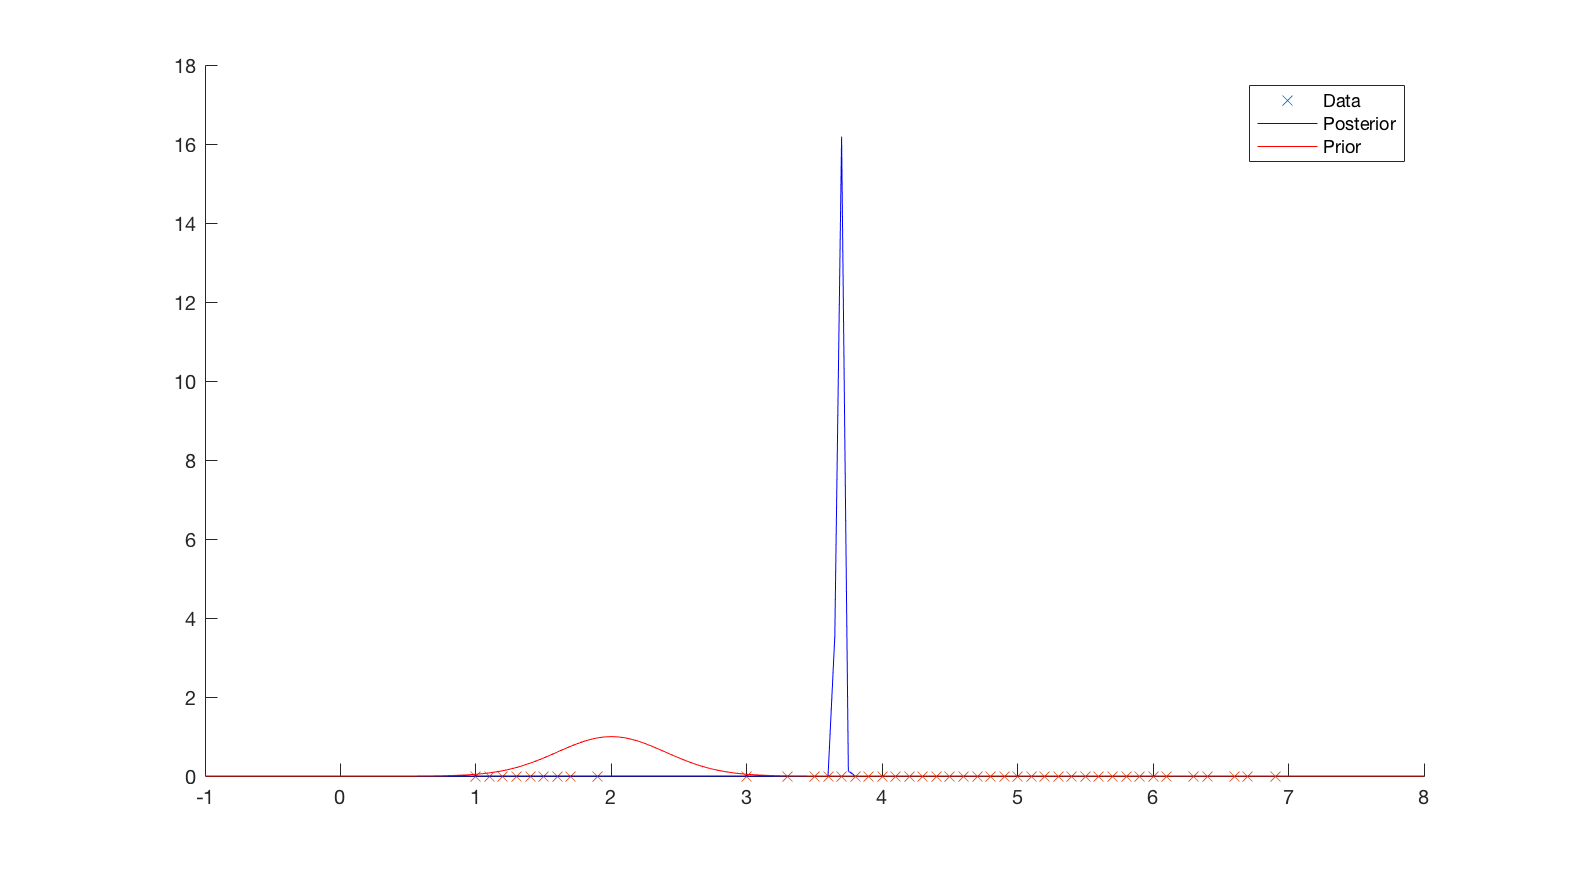
\includegraphics[width=\linewidth]{../../pracs/prac11/q1_graph}
    \centering
    \caption{Model prior and posterior distributions}
\end{figure}

\end{document}
